% =================================================================================================
% File:			content_files.tex
% Description:	Defiinisce i capitoli presenti nel documento
% Created:		2015-04-21
% Author:		Tesser Paolo
% Email:		tesser.paolo@mashup-unipd.it
% =================================================================================================
% Modification History:
% Version		Modifier Date		Change											Author
% 0.0.1 		2015-04-21 			creazione struttura								Tesser Paolo
% =================================================================================================
%

% DEFINIZIONE FUNZIONE GLOSSARIO
% Questa funzione si occupa di disegnare la lettera per ogni sezione del glossario


% DEFINIZIONE DEI CONTENUTI DEL DOCUMENTO 

% =================================================================================================
% File:			introduzione.tex
% Description:	Defiinisce la sezione relativa al capitolo introduttivo del documento
% Created:		2015-04-21
% Author:		Tesser Paolo
% Email:		tesser.paolo@mashup-unipd.it
% =================================================================================================
% Modification History:
% Version		Modifier Date		Change											Author
% 0.0.1 		2015-04-21 			creato scheletro doc e primo abbozzo			Tesser Paolo
% =================================================================================================
%

% CONTENUTO DEL CAPITOLO

\section{Introduzione} % (fold)
\label{sec:introduzione}
	\subsection{Scopo del documento} % (fold)
	\label{sub:scopo_del_documento}
	Questo documento ha come scopo quello di illustrare le procedure da seguire per svolgere le operazioni previste per l'utente amministratore relative al prodotto \projectName. All'utilizzatore non è chiesta nessuna particolare conoscenza informatica. Alcune operazioni richiedono però che esso abbia dimestichezza con i social network e con le possibilità che offrono.
	% subsection scopo_del_documento (end)

	\subsection{Scopo del prodotto} % (fold)
	\label{sub:scopo_del_prodotto}
	\productScope
	% subsection scopo_del_prodotto (end)

	\subsection{Prerequisiti} % (fold)
	\label{sub:prerequisiti}
	TODO (prendere spunto dagli Steakholders)
	% subsection prerequisiti (end)

	\subsection{Problemi e malfunzionamenti} % (fold)
	\label{sub:problemi_e_malfunzionamenti}
	TODO (prendere spunto dagli Steakholders)
	% subsection problemi_e_malfunzionamenti (end)

	\subsection{Glossario} % (fold)
	\label{sub:glossario}
	TODO (forse servirà inserire il glossario in appendice in quanto agli utenti non viene fornito l'altro Glossario) \newline
	\glossarioDesc
	% subsection glossario (end)

	\subsection{Riferimenti} % (fold)
	\label{sub:riferimenti}
		\subsubsection{Normativi} % (fold)
		\label{ssub:normativi}
			\begin{itemize}
				\item \textbf{Analisi dei Requisiti}: \docNameVersionAdR
				\item \textbf{Specifica Tecnica}: \docNameVersionST
			\end{itemize}
		% subsubsection normativi (end)

		\subsubsection{Informativi} % (fold)
		\label{ssub:informativi}
			\begin{itemize}
				\item \textbf{TODO}: TODO;
			\end{itemize}
		% subsubsection informativi (end)
	% subsection riferimenti (end)
% section introduzione (end)
% section introduzione (end) \newpage \clearpage
% =================================================================================================
% File:			istruzioni_utilizzo.tex
% Description:	Definisce la sezione relativa ad un capitolo del documento
% Created:		2015-04-21
% Author:		Santacatterina Luca
% Email:		santacatterina.luca@mashup-unipd.it
% =================================================================================================
% Modification History:
% Version		Modifier Date		Change											Author
% 0.0.1 		2015-05-24 			inizio stesura sezione capitolo					Santacatterina Luca
% =================================================================================================
%

% CONTENUTO DEL CAPITOLO
\section{Istruzioni per l'utilizzo} % (fold)
\label{sec:istruzioni_per_l_utilizzo}


	\subsection{Requisiti necessari} % (fold)
	\label{sec:requisiti_necessari}
		Prima di iniziare l'utilizzo del software \projectName{} lato amministratore leggere attentamente la corretta procedura d'utilizzo nel \docNameVersionMU.\newline
		Di seguito vengono riportati tutti i requisiti hardware\gloss{} e software\gloss{} necessari per poter utilizzare tutte le funzionalità del prodotto.\newline
		Per poter accedere all'applicazione \projectName, è necessario verificare che sia attiva una connessione ad Internet a banda larga\gloss{} in grado di collegarsi via URL\gloss{} e possedere le credenziali\gloss{} di accesso.

		\subsubsection{Requisiti hardware} % (fold)
		\label{sec:requisiti_hardware}
			L'applicazione è sviluppata per funzionare sia su dispositivi fissi che mobili quali tablet e smartphone.\newline
			Per usufruire di tutte le funzionalità si raccomanda l'utilizzo dell'applicativo tramite computer desktop e notebook.\newline
			È necessario operare da una postazione di lavoro dotata dei requisiti tecnici elencati di seguito:
			\begin{itemize}
				\item \textbf{Risoluzione}:
				\begin{itemize}
					\item per postazioni desktop risoluzioni maggiori di 1024x768;
					\item per postazioni mobile risoluzioni maggiori di 1024x600;
				\end{itemize}
			\end{itemize}
		% section Requisiti hardware (end)

		\subsubsection{Requisiti software} % (fold)
		\label{sec:requisiti_software}
			Affinchè l'applicazione possa funzionare correttamente tramite computer desktop è necessario disporre di uno dei seguenti browser\gloss{}:
			\begin{itemize}
				\item \textbf{Google Chrome}: versione 42 o superiore;
				\item \textbf{Internet Explorer}: versione 11 o superiore;
				\item \textbf{Mozilla Firefox}: versione 38 o superiore;
				\item \textbf{Safari}: versione 8.0.6 o superiore.
			\end{itemize}

			Affinchè l'applicazione possa funzionare correttamente tramite dispositivi mobile è necessario disporre di uno dei seguenti browser\gloss{}:
			\begin{itemize}
				\item \textbf{Google Chrome}:
				\begin{itemize}
					\item per Android versione 42 o superiore;
					\item per iOS versione 42 o superiore;
				\end{itemize}
			\item \textbf{Safari}: per iOS versione 8.0.6 o superiore.
			\end{itemize}

			Per una corretta visualizzazione è necessario:
			\begin{itemize}
				\item abilitare l'utilizzo dei cookies\gloss{}. Per le istruzioni fare riferimento alle specifiche funzionali di ciascun browser\gloss{};
				\item blocco dei pop-up\gloss{} disattivato. Per le istruzioni fare riferimento alle specifiche funzionali di ciascun browser\gloss{}.
			\end{itemize}
		% section Requisiti software (end)

		\subsubsection{Dati richiesti} % (fold)
		\label{sec:dati_richiesti}
			Per poter utilizzare l'applicazione è necessario fornire i seguenti dati:
			\begin{itemize}
				\item \textbf{Dati personali}: si richiedono dati personali per poter contattare in caso di guasti o notifiche;
				\item \textbf{Email}: si richiede un indirizzo di posta elettronica attivo su cui ricevere messaggi email.
			\end{itemize}
		% section Dati richiesti (end)

		\subsubsection{Installazione} % (fold)
		\label{sec:installazione}
			L'applicazione non prevede l'installazione di ulteriori componenti aggiuntivi per il regolare funzionamento.
			L'indirizzo per il collegamento all'applicazione è:\newline
			\begin{center}
				\url{http://mashup-unipd.github.io/}
			\end{center}
			Non appena la pagina si sarà caricata, sarà possibile effettuare l'accesso all'applicativo.
		% section installazione (end)

		\subsubsection{Comunicazioni malfunzionamenti} % (fold)
		\label{sec:installazione}
			Se durante l'utilizzo dell'applicazione \projectName{} si dovessero riscontrare problemi o malfunzionamenti, si invitano gli utilizzatori a segnalare l'errore inviando una email all'indirizzo:
			\begin{center}
				\url{info@mashup-unipd.it}
			\end{center}
			Nella mail di segnalazione si dovranno riportare:
			\begin{itemize}
				\item username ed email forniti in fase di registrazione dell'applicazione (ATTENZIONE: non è richiesta la password di autenticazione\gloss{});
				\item versione di browser\gloss{} e sistema operativo\gloss{} utilizzato. Nel caso di dispositivi mobile il modello utilizzato;
				\item descrizione dettagliata del problema riscontrato e relativi errori visualizzati;
			\end{itemize}
			Prima di aprire una richiesta di assistenza si consiglia di effettuare operazioni di pulizia dei file cookies\gloss{}. Per le istruzioni fare riferimento alle specifiche funzionali di ciascun browser\gloss{}.
		% section comunicazioni malfunzionamenti (end)

	% section Requisiti necessari (end)

% section Istruzioni per l'utilizzo (end)
 \newpage \clearpage
% =================================================================================================
% File:			registrazione_e_autenticazione.tex
% Description:	Definisce la sezione relativa ad un capitolo del documento
% Created:		2015-04-21
% Author:		Santacatterina Luca
% Email:		santacatterina.luca@mashup-unipd.it
% =================================================================================================
% Modification History:
% Version		Modifier Date		Change											Author
% 0.0.1 		2015-05-24 			inizio stesura sezione capitolo					Santacatterina Luca
% =================================================================================================
%

% CONTENUTO DEL CAPITOLO
\section{Autenticazione} % (fold)
\label{sec:autenticazione}
	In questa sezione saranno descritte le funzionalità di autenticazione\gloss{} fornite all'utente nella fase iniziale.


		\subsection{Autenticazione utente amministratore} % (fold)
		\label{sec:autenticazione_utente}
			Per effettuare l'autenticazione\gloss{} all'applicazione ci si deve collegare al sito tramite l'URL\gloss{} riportato nel capitolo \ref{sec:installazione} e si devono inserire le credenziali:
			\begin{itemize}
				\item Email;
				\item Password.
			\end{itemize}
			\begin{figure}[H]
				\centering
				\centerline{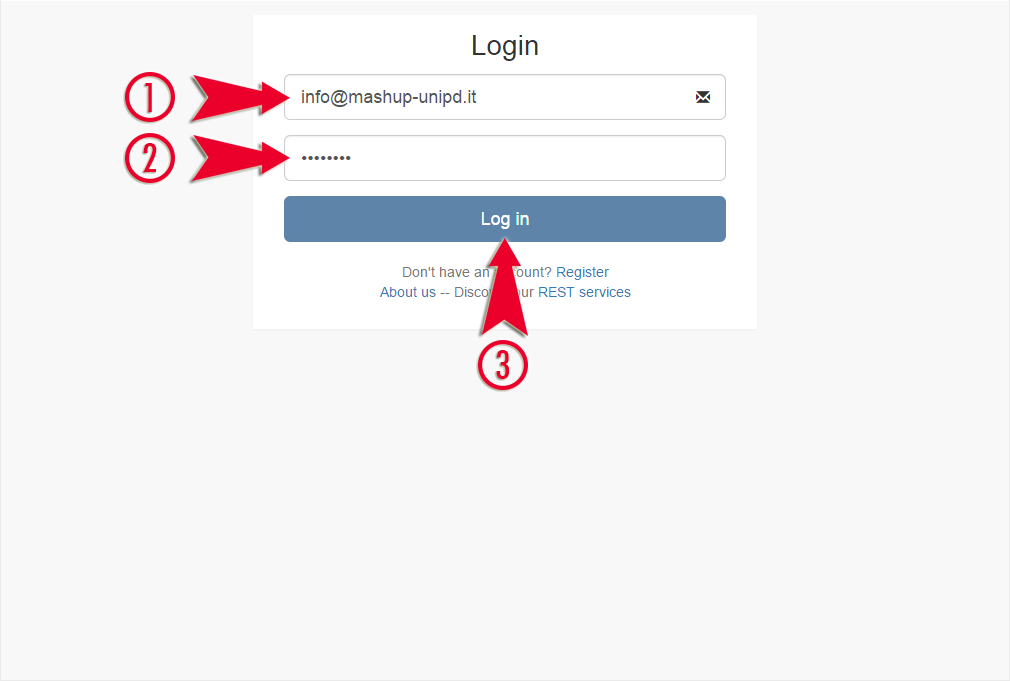
\includegraphics[width=14cm]{images/autenticazione_utente.png}}
				\caption{Autenticazione utente amministratore}
				\label{fig:registrazione_utente_accesso}
			\end{figure}
			\pagebreak
			\noindent
			Dopo aver inserito i dati di autenticazione\gloss{} (Figura \ref{fig:registrazione_utente_accesso}) sarà possibile premere il pulsante \textbf{Login}\gloss{} e quindi si verrà collegati alla dashboard\gloss{} dell'applicazione (Figura: \ref{fig:dashboard})
			\begin{figure}[H]
				\centering
				\centerline{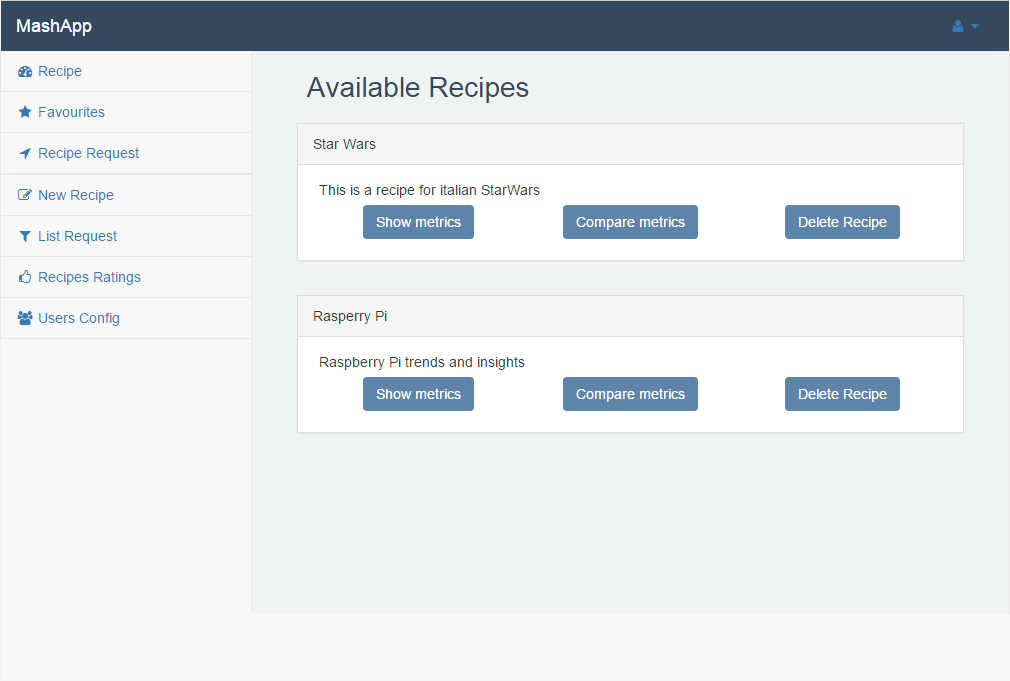
\includegraphics[width=19cm]{images/dashboard_amministratore.png}}
				\caption{Dashboard applicazione}
				\label{fig:dashboard}
			\end{figure}
		% section Autenticazione utente (end)


	% section Registrazione (end)

% section Registrazione e autenticazione (end) \newpage \clearpage
% =================================================================================================
% File:			gestione_contenuti.tex
% Description:	Definisce la sezione relativa ad un capitolo del documento
% Created:		2015-04-25
% Author:		Santacatterina Luca
% Email:		santacatterina.luca@mashup-unipd.it
% =================================================================================================
% Modification History:
% Version		Modifier Date		Change											Author
% 0.0.1 		2015-05-245			inizio stesura sezione capitolo					Santacatterina Luca
% =================================================================================================
%

% CONTENUTO DEL CAPITOLO

\section{Gestione contenuti} % (fold)
\label{sec:gestione_contenuti}
	Dopo aver eseguito le istruzioni per l'autenticazione\gloss{} viene visualizzata la dashboard\gloss{} dell’applicazione.\newline
	Nella schermata principale della dashboard\gloss{} vengono visualizzati in riquadri le \textbf{recipes}\gloss{} disponibili nel sistema (Figura: \ref{fig:ricette_disponibili}), mentre nella sinistra dell'applicazione è disponibile il menù principale di gestione (Figura: \ref{fig:menu_principale_utente})
	\begin{figure}[H]
		\centering
		\centerline{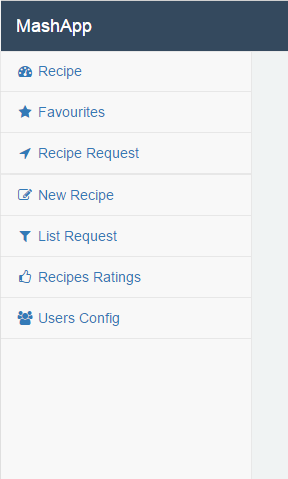
\includegraphics[width=6cm]{images/menu_principale_amministratore.png}}
		\caption{Menù principale amministratore}
		\label{fig:menu_principale_utente}
	\end{figure}

% section Gestione contenuti (end) \newpage \clearpage
% =================================================================================================
% File:			gest_recipe.tex
% Description:	Defiinisce la sezione relativa ad un capitolo del documento
% Created:		2015-04-21
% Author:		Tesser Paolo
% Email:		tesser.paolo@mashup-unipd.it
% =================================================================================================
% Modification History:
% Version		Modifier Date		Change											Author
% 0.0.1 		2015-04-21 			creato scheletro doc							Tesser Paolo
% =================================================================================================
%

% CONTENUTO DEL CAPITOLO
\section{Gestione delle Recipe} % (fold)
\label{sec:gestione_delle_recipe}


	\subsection{Contenuti Sezione} % (fold)
	\label{sub:contenuti_sezione}
		All'utente amministratore sono concessi permessi di modifica e gestione delle recipe\gloss{}.
		La gestione prevede:
		\begin{itemize}
			\item Aggiunta di una nuova recipe\gloss{};
			\item Eliminazione di una o più recipe\gloss{};
			\item Visualizzazione classifica delle recipe\gloss{};
		\end{itemize}


	\subsection{Aggiunta di una nuova recipe}
		Dal menu principale situato nella dashboard\gloss{} del sistema è possibile visualizzare l'elenco delle recipe\gloss{} premendo sull'apposito pulsante \textbf{Recipe}.\newline
		Tramite il pulsante \textbf{New Recipe} è possibile accedere alla nuova pagina (Figura: \ref{fig:aggiunta_nuova_recipe}) per l'inserimento guidato di nuove recipe\gloss{}.
		\begin{figure}[H]
			\centering
			\centerline{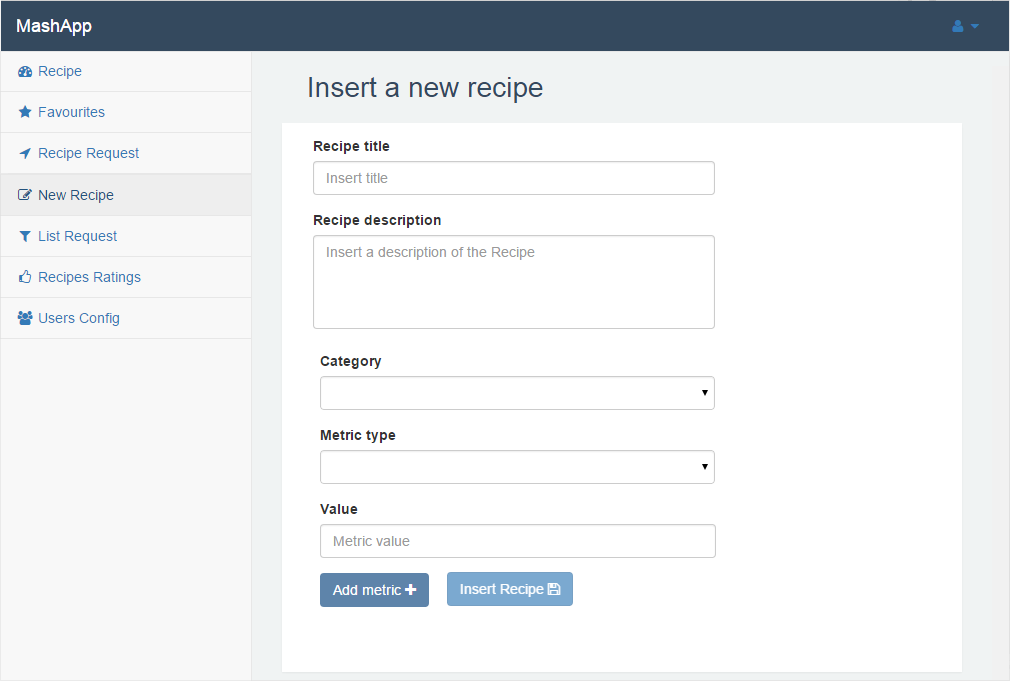
\includegraphics[width=14cm]{images/nuova_ricetta.png}}
			\caption{Aggiunta nuova recipe}
			\label{fig:aggiunta_nuova_recipe}
		\end{figure}
		Per aggiungere una nuova nuova recipe\gloss{} è necessario compilare tutti i campi del form\gloss{} (Figura: \ref{fig:aggiunta_nuova_recipe}) con i seguenti dati:
		\begin{itemize}
			\item Nome della recipe;
			\item Descrizione della recipe;
			\item Parametri relativi alla recipe dipendenti dal/dai social network di interesse;
		\end{itemize}
		È possibile selezionare uno o più social network e uno o più parametri per ciascuna selezione.\newline
		Al termine della procedura guidata è necessario premere il pulsante di \textbf{Insert Recipe} per salvare le modifiche ed aggiungere così la recipe\gloss{} al sistema.
	% END


	\subsection{Eliminazione Recipe}
		L'amministratore può eliminare una recipe\gloss{} e tutti i dati ad essa associati dal sistema.\newline
		Per accedere all'area dedicata della dashboard\gloss{} si deve premere sul pulsante \textbf{Recipe}\gloss{}. Dall'elenco delle recipe\gloss{} (Figura: \ref{fig:dashboard}) è disponibile il pulsante \textbf{Delete recipe}.
		L'eliminazione della recipe è istantanea si può così procedere ad una nuova operazione.
	% END

	
	\subsection{Visualizzazione classifica recipe}
		L'utente amministratore può visualizzare la classifica (Figura: \ref{fig:votazioni_ricette}) delle recipe\gloss{} in ordine dalla più apprezzata alla meno apprezzata.\newline
		Per accedere alla sezione è richiesto di premere l'apposito pulsante \textbf{Recipes Ratings} dal menu principale nella dashboard\gloss{}.\newline
		\begin{figure}[H]
			\centering
			\centerline{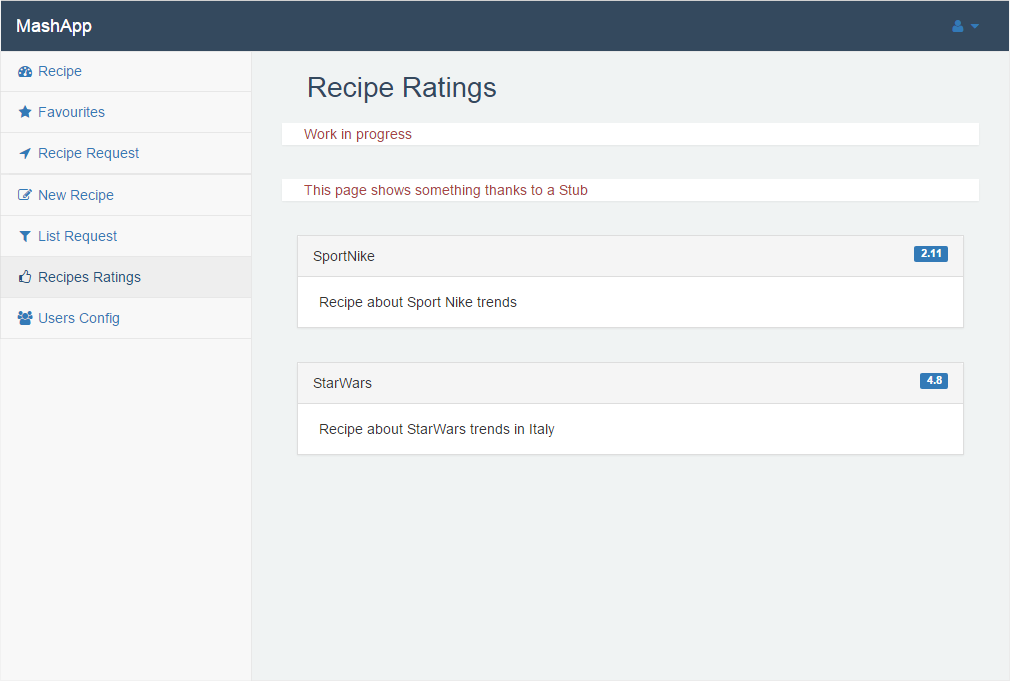
\includegraphics[width=14cm]{images/votazioni_ricette.png}}
			\caption{Punteggi recipes}
			\label{fig:votazioni_ricette}
		\end{figure}
		Nel caso in cui nessun utente abbia ancora dato un giudizio sulle recipe presenti nel sistema, la classifica risulterà vuota.\newline
		Un messaggio avviserà l'utente amministratore se questa situazione dovesse verificarsi.
	% END


% section Gestione delle Recipe (end) \newpage \clearpage
% =================================================================================================
% File:			gest_richieste.tex
% Description:	Defiinisce la sezione relativa ad un capitolo del documento
% Created:		2015-04-21
% Author:		Tesser Paolo
% Email:		tesser.paolo@mashup-unipd.it
% =================================================================================================
% Modification History:
% Version		Modifier Date		Change											Author
% 0.0.1 		2015-04-21 			creato scheletro doc							Tesser Paolo
% =================================================================================================
%

% CONTENUTO DEL CAPITOLO
\section{Gestione richieste recipe} % (fold)
\label{sec:gest_richieste}


	\subsection{Contenuti Sezione} % (fold)
	\label{sub:contenuti_sezione}
		L'amministratore può provvedere ad approvare o respingere l'inserimento di una nuova recipe\gloss{} proposta da un utente.\newline
		Vengono messe a disposizione dell'amministratore le seguenti funzioni:
		\begin{itemize}
			\item \textbf{See Details}: visualizza i dettagli della recipe richiesta (Figura: \ref{fig:richiesta_ricette}, rif. 1);
			\item \textbf{Discard}: disapprova la richiesta (Figura: \ref{fig:richiesta_ricette}, rif. 2);
			\item \textbf{Approve}: approva la richiesta di aggiunta (Figura: \ref{fig:richiesta_ricette}, rif. 3);
		\end{itemize}
		E' possibile visualizzare l'elenco delle recipe\gloss{} in attesa di approvazione (Figura: \ref{fig:richiesta_ricette}).
		\begin{figure}[H]
			\centering
			\centerline{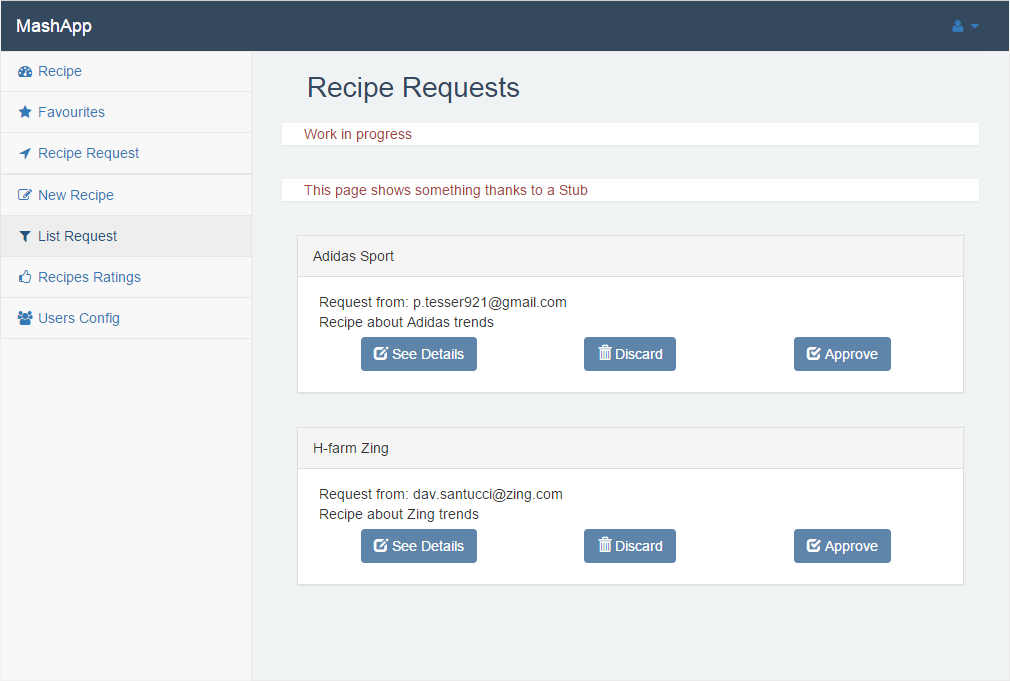
\includegraphics[width=14cm]{images/richiesta_ricette.png}}
			\caption{Approvazioni e eliminazione richieste utente}
			\label{fig:richiesta_ricette}
		\end{figure}


	\pagebreak
	\subsection{Visualizza elenco richieste}
		L'utente amministratore può visualizzare un elenco delle richieste delle recipe\gloss{} (Figura: \ref{fig:richiesta_ricette}) che sono state inviate dagli utenti normali e non ancore marcate come \textbf{chiuse}.\newline
		Per accedere all'elenco delle richieste (Figura: \ref{fig:richiesta_ricette}), selezionare l'apposito pulsante \textbf{List Request} dal menu principale della dashboard\gloss{} (Figura: \ref{fig:dashboard}).
	% END
	

	\subsection{Visualizza dettagli richiesta}
		L'utente amministratore può visualizzare tutti i dettagli di una richiesta, dopo aver premuto il pulsante \textbf{See Details} (Figura: \ref{fig:richiesta_ricette}, rif. 1) dall'elenco delle richieste.\newline
		I dettagli di una richiesta includono:
		\begin{itemize}
			\item Il nome dell'utente che l'ha inoltrata;
			\item Il titolo della richiesta;
			\item La descrizione della richiesta;
			\item L'identificativo presente sul social network.
		\end{itemize}
		Un utente amministratore può accettare o respingere una richiesta.\newline
		Può inoltre modificare il titolo o la descrizione qualora li ritenesse inopportuni.
	% END
	
	
	\subsection{Modifica richiesta Recipe}
		L'utente amministratore può modificare titolo e descrizione della richiesta per renderla più efficace da comprendere per gli altri amministratori.
		Per eseguire questa operazione occorre identificare dall'elenco delle richieste recipe\gloss{} e premere sul pulsante \textbf{See Details} (Figura: \ref{fig:richiesta_ricette}, rif. 2).
		I parametri che si possono modificare sono i seguenti:
		\begin{itemize}
		 	\item Il titolo della richiesta;
		 	\item La descrizione della richiesta;
		\end{itemize}
		Una volta terminate le modifiche è necessario selezionare il pulsante \textbf{Save} affinché queste siano attive nel sistema.
	% END

	\pagebreak
	\subsection{Accettazione richiesta}
		L'utente amministratore, una volta controllata la validità della recipe\gloss{} richiesta, potrà accettarla in modo che venga inserita nel sistema\gloss{}.\newline
		Per svolgere questa operazione occorre accedere innanzitutto all'elenco delle richieste recipe\gloss{} (Figura: \ref{fig:richiesta_ricette}) dal Menu principale della dashboard\gloss{} (Figura: \ref{fig:dashboard}).\newline
		Per confermare la richiesta basta solamente premere il pulsante \textbf{Approve} (Figura: \ref{fig:richiesta_ricette}, rif. 3) presente nell'elenco.\newline
		E' necessario confermare l'operazione selezionando il pulsante \textbf{Save} quando richiesto.\newline
		Il sistema a questo punto crea una recipe\gloss{} utilizzando i dati forniti dall'utente e confermati con l'operazione appena descritta.\newline
		Una richiesta marcata come accettata viene rimossa dall'elenco delle richieste e non più visualizzata dagli amministratori.\newline
	% END


	\subsection{Respinta richiesta}
		L'utente amministratore può decidere di rifiutare la richiesta.
		Per svolgere questa operazione è necessario accedere innanzitutto all'elenco delle richieste recipe\gloss{} (Figura: \ref{fig:richiesta_ricette}) dal Menu principale della dashboard\gloss{} (Figura: \ref{fig:dashboard}).\newline
		Per eliminare la richiesta è necessario premere il pulsante \textbf{Discard} (Figura: \ref{fig:richiesta_ricette}, rif. 2). In seguito è necessario confermare l'operazione selezionando il pulsante \textbf{Save} quando richiesto.\newline
		Una richiesta marcata come respinta viene rimossa dall'elenco delle richieste e non più visualizzata dagli altri amministratori.
	% END


% section Gestione degli utenti (end) \newpage \clearpage
% =================================================================================================
% File:			amm_utenti.tex
% Description:	Defiinisce la sezione relativa ad un capitolo del documento
% Created:		2015-04-21
% Author:		Tesser Paolo
% Email:		tesser.paolo@mashup-unipd.it
% =================================================================================================
% Modification History:
% Version		Modifier Date		Change											Author
% 0.0.1 		2015-04-21 			creato scheletro doc							Tesser Paolo
% =================================================================================================
%

% CONTENUTO DEL CAPITOLO
\section{Gestione degli utenti} % (fold)
\label{sec:gestione_utenti}
	

	\subsection{Contenuti Sezione} % (fold)
	\label{sub:contenuti_sezione}
		All'utente amministratore sono concessi permessi di gestione degli utenti.
		La gestione prevede le seguenti funzionalità:
		\begin{itemize}
			\item Visualizzazione dell'elenco di tutti utenti registrati sull'applicazione (Figura: \ref{fig:configurazione_utenti});
			\item Modifica permessi utente (Figura: \ref{fig:configurazione_utenti}, rif. 2);
			\item Eliminazione profilo utente (Figura: \ref{fig:configurazione_utenti}, rif. 3);
		\end{itemize}
		\begin{figure}[H]
			\centering
			\centerline{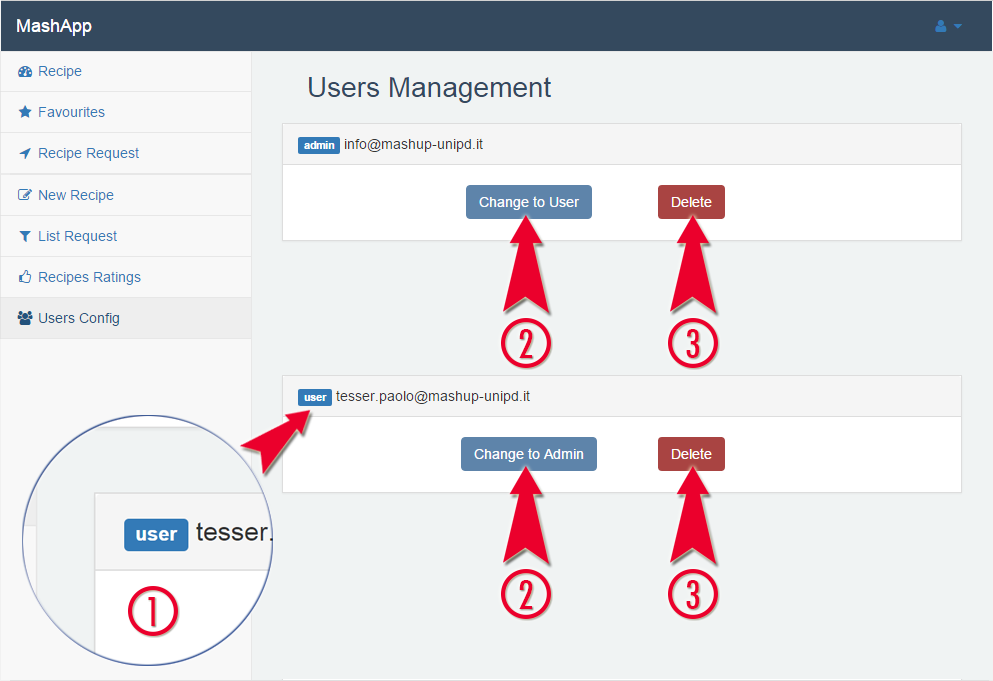
\includegraphics[width=14cm]{images/configurazione_utenti.png}}
			\caption{Gestione utenti}
			\label{fig:configurazione_utenti}
		\end{figure}
	% END

	\pagebreak
	\subsection{Visualizzazione elenco utenti}
		L'utente amministratore può visualizzare l'elenco (Figura: \ref{fig:configurazione_utenti}) di tutti gli utenti registrati nel sistema selezionando l'apposito pulsante dal menu principale (Figura: \ref{fig:menu_principale_utente}) situato nella Home Page della dashboard\gloss{} (Figura: \ref{fig:dashboard}).\newline
		In questo elenco (Figura: \ref{fig:configurazione_utenti}) è possibile visualizzare tutti i dati di ciascun utente, modificare  i suoi permessi oppure eliminare un utente, purché esso non sia un amministratore a sua volta.\newline
		L'identificazione del tipo di permessi è visualizzata per ogni singolo utente (Figura: \ref{fig:configurazione_utenti}, rif. 3).
	% END	

	
	\subsection{Modifica permessi utente}
		L'utente amministratore può abilitare i permessi di amministratore ad un utente diverso da se stesso.\newline
		Per effettuare questa operazione è necessario accedere all'elenco degli utenti (Figura: \ref{fig:configurazione_utenti}) premendo l'apposito pulsante dal menu principale di amministrazione (Figura: \ref{fig:menu_principale_utente}) dell'applicazione situato nella Home Page della dashboard (Figura: \ref{fig:dashboard}).
		La procedura prevede l'individuazione dell'utente nel sistema e la relativa pressione del pulsante \textbf{Change to admin} (Figura: \ref{fig:configurazione_utenti}, rif. 1).\newline
		Una volta effettuata la selezione è richiesto di premere il pulsante di conferma dell'operazione per rendere effettive le modifiche.
	% END

	
	\subsection{Eliminazione utente}
		L'utente amministratore può eliminare un utente diverso da se stesso dal sistema.\newline
		Per effettuare questa operazione è necessario accedere all'elenco degli utenti (Figura: \ref{fig:configurazione_utenti}) premendo l'apposito pulsante dal menu principale di amministrazione Figura: \ref{fig:menu_principale_utente}) dell'applicazione situato nella Home Page della dashboard (Figura: \ref{fig:dashboard}).
		La procedura prevede l'individuazione dell'utente nel sistema e la relativa pressione del pulsante \textbf{Delete} (Figura: \ref{fig:configurazione_utenti}, rif. 2).\newline
		Una volta effettuata la selezione è richiesto di premere il pulsante di conferma dell'operazione di eliminazione per rendere effettive le modifiche.\newline
		ATTENZIONE: l'operazione di eliminazione utente non è reversibile.
	% END
		

% section Gestione degli utenti (end) \newpage \clearpage
\appendix
% =================================================================================================
% File:			glossario.tex
% Description:	Defiinisce la sezione relativa ad un capitolo del documento
% Created:		2015-05-25
% Author:		Santacatterina Luca
% Email:		santacatterina.luca@mashup-unipd.it
% =================================================================================================
% Modification History:
% Version		Modifier Date		Change											Author
% 0.0.1 		2015-05-25 			prima abbozza glossario							Santacatterina Luca
% =================================================================================================
%

% CONTENUTO DEL CAPITOLO
\section{Glossario} % (fold)
\label{sec:glossario}


	\section*{\Huge A} % (fold)
		\begin{itemize}
			\item \textbf{Android:} sistema operativo per sistemi mobile sviluppato da Google e basato su kernel Linux. Sviluppato principalmente per dispositivi touchscreen quali smartphone e tablet, lo si può trovare con interfacce utenti specializzate per televisori (Android TV), automobili (Android Auto), orologi da polso (Android Wear) e occhiali (Google Glass);
			\item \textbf{API:} acronimo di Application Programming Interface, è un insieme di routine, protocolli e strumenti che consentono ai software di interagire tra di loro. Funziona come un'interfaccia tra software differenti facilitandone la loro interazione, allo stesso modo in cui un'interfaccia utente facilita l'interazione tra uomo e computer;
			\item \textbf{Autenticazione:} verifica attraverso un sistema automatico di interrogazione e risposta in grado di stabilire un collegamento autorizzato e valido.;
		\end{itemize}
	% section a (end)


	\section*{\Huge B} % (fold)
		\begin{itemize}
			\item \textbf{Browser:} programma che consente di visualizzare i contenuti delle pagine dei siti web e di interagire con essi, permettendo così all’utente di navigare in internet. Il browser è in grado di interpretare l’HTML (il codice con il quale sono scritte la maggior parte delle pagine web) e di visualizzarlo. I browser attualmente più noti e diffusi sono Internet Explorer, Mozilla Firefox, Google Chrome, Safari e Opera;
		\end{itemize}
	% section b (end)


	\section*{\Huge C} % (fold)
		\begin{itemize}
			\item \textbf{Cookies:} files di piccole dimensioni all'interno del dispositivo che contengono delle informazioni registrate e fungono da identificatori automatici per riscontrare i visitatori e le loro sessioni di visita nel sito;
			\item \textbf{Credenziali:} dati in possesso dall'utente, da questi conosciuti o ad essa univocamente correlati, utilizzati per l'autenticazione informatica;
		\end{itemize}
	% section c (end)


	\section*{\Huge D} % (fold)
		\begin{itemize}
			\item \textbf{Database:} collezione di dati organizzata. Le informazioni contenute in esso sono strutturate e collegate tra loro mediante un particolare modello logico in modo tale da consentire l'organizzazione efficiente dei dati stessi e l'interfacciamento con le richieste dell'utente attraverso le query di interrogazione;
			\item \textbf{Dashboard:} interfaccia grafica che organizza e presenta le informazioni in modo semplice, intuitivo, immediato ed ordinato. Consente all'utente di consultare il pannello in modo ordinato;
		\end{itemize}
	% section d (end)


	\section*{\Huge F} % (fold)
		\begin{itemize}
			\item \textbf{Form:} nota anche come modulo web, all'interno di una pagina web permette ad un utente di inserire dei dati da inviare al server per essere poi processati. Una form può assumere l'aspetto di un modulo cartaceo poiché tipicamente composto da checkbox, radio button e campi di testo. Sono utilizzate, per esempio, per inserire i dati di spedizione o della carta di credito per l'acquisto di un prodotto via internet, o possono essere utilizzate per recuperare i risultati di una ricerca da un motore di ricerca;
		\end{itemize}
	% section f (end)


	\section*{\Huge H} % (fold)
		\begin{itemize}
			\item \textbf{Hardware:} Tradotto letteralmente dall'inglese significa ferramenta. Termine generico per indicare le componenti fisiche (device, dispositivi) di un elaboratore quali i circuiti elettronici, chip, schede, disk drive, stampanti, mouse, lettori CD-ROM, monitor, tastiera ecc;
		\end{itemize}
	% section h (end)


	\section*{\Huge I} % (fold)
		\begin{itemize}
			\item \textbf{Internet a banda larga:} in lingua inglese indicata con il termine broadband. Nel campo delle telecomunicazioni e informatica, indica generalmente la trasmissione e ricezione di dati informativi, inviati e ricevuti simultaneamente in maggiore quantità, sullo stesso cavo o mezzo radio grazie all'uso di mezzi trasmissivi e tecniche di trasmissione che supportino e sfruttino un'ampiezza di banda superiore ai precedenti sistemi di telecomunicazioni detti invece a banda stretta;
		\end{itemize}
	% section h (end)


	\section*{\Huge L} % (fold)
		\begin{itemize}
			\item \textbf{Login:} procedura di accesso al sistema informatico. Prevede l'inserimento di un codice identificativo e di una parola d'ordine da parte dell'utente;
			\item \textbf{Logout:} procedura di uscita dal sistema informatico. Non prevede l'inserimento di ulteriori informazioni;
		\end{itemize}
	% section f (end)


	\section*{\Huge P} % (fold)
		\begin{itemize}
			\item \textbf{Pop-up:} ingrandimenti di parti di applicazione su finestra dedicata. Presentano nel contesto funzione di attrazione dell'attenzione dei visitatori;
		\end{itemize}
	% section p (end)


	\section*{\Huge R} % (fold)
		\begin{itemize}
			\item \textbf{Recipe:} collezioni di informazioni raccolte dai social network periodicamente e generate dall'applicativo server-side. Vengono utilizzate per generare e aggiornare i dati e i grafici dagli utenti;
			\item \textbf{Responsive:} tipo di design utilizzato nei siti web che permette ai siti di adattarsi graficamente in modo automatico al dispositivo coi quali vengono visualizzati, riducendo al minimo la necessità per l'utente di ridimensionamento e scorrimento dei contenuti;
			\item \textbf{REST:} acronimo di REpresentational State Transfer, è un tipo di architettura software per il Word Wide Web molto usato nell'HTTP. REST infatti si riferisce ad un insieme di principi di architetture di rete, i quali delineano come le risorse sono definite e indirizzate;
			\end{itemize}
	% section r (end)


	\section*{\Huge S} % (fold)
		\begin{itemize}
			\item \textbf{Screenshot:} processo di acquisizione istantanea che consente di salvare sotto forma di immagini ciò che viene visualizzato sullo schermo di un computer;
			\item \textbf{Software:} termine generico che intende un programma, quindi un insieme di istruzioni (algoritmi e dati) che possono essere eseguite dalla CPU. Se le istruzioni devono essere compilate, ossia sono istruzioni ad alto livello si parla di codice sorgente del programma. Se il software viene utilizzato direttamente dagli utenti si parla di applicazione. In genere se il software viene utilizzato dal sistema operativo lo si indica con il termine software di sistema;
		\end{itemize}
	% section s (end)


	\section*{\Huge T} % (fold)
		\begin{itemize}
			\item \textbf{Token:} sequenza di caratteri alfanumerici generata dal server e fornita all'utente singolarmente. Le informazioni necessarie risiedono direttamente nel computer dell'utente, e non in un oggetto esterno;
		\end{itemize}
	% section t (end)


	\section*{\Huge U} % (fold)
		\begin{itemize}
			\item \textbf{URL:} con il termine URL si identifica l’acronimo Uniform Resource Locator. Definito da una sequenza di caratteri che identifica univocamente l’indirizzo di una risorsa in Internet, come un documento o un’immagine;
		\end{itemize}
	% section u (end)


	\section*{\Huge V} % (fold)
		\begin{itemize}
			\item \textbf{View:} dati e grafici creati dagli utenti autenticati utilizzando le recipe;
		\end{itemize}
	% section v (end)


% section Glossario (end) \newpage \clearpage